\documentclass[../../entrega.tex]{subfiles}
\begin{document}

\subsection{Inciso (b)}
El archivo \texttt{1.b.jl} contiene el código necesario para replicar las figuras 1 y 2 del artículo de \textcite{werning_recalculating_2024}, que se pueden ver en las figuras \ref{fig:figure1} y \ref{fig:figure2} respectivamente.
La figura \ref{fig:figure1} muestra la curva de Laffer tradicional (la línea punteada de abajo) y la curva alternativa (la línea sólida de arriba) usando la demanda de dinero de \textcite{sargent_unpleasant_1981}.
La figura \ref{fig:figure2} muestra los equilibrios para un ejemplo simple que desarrolla Werning.
Enfocándose en equilibrios con inflación constante en $\pi_\infty$ a partir de $t = 2$, computa $\pi_{0, 1}$ como función de $\pi_\infty$.
El conjunto de equilibrios es representado por la curva sólida, cuyas regiones decrecientes y crecientes corresponden a los lados izquierdo y derecho de la curva de Laffer de la figura \ref{fig:figure1} respectivamente.

\textcolor{red}{TODO: flesh out explanation}

\begin{figure}[!htb]
    \centering
    \includegraphics[width=0.7\textwidth]{figure1.pdf}
    \caption{Curvas de Laffer en el ejemplo ``espectacular'' de Sargent y Wallace}
    \label{fig:figure1}
\end{figure}
\begin{figure}[!htb]
    \centering
    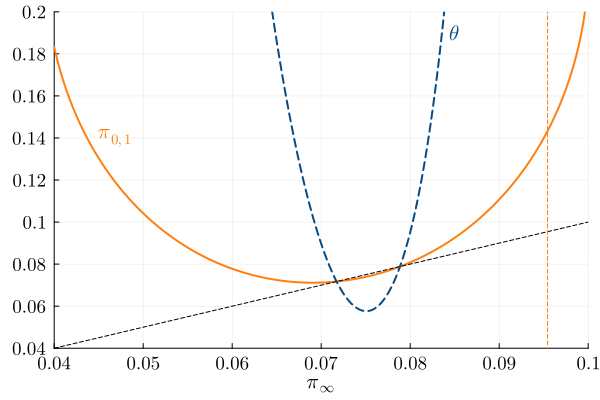
\includegraphics[width=0.7\textwidth]{figure2.pdf}
    \caption{Equilibrios para un ejemplo simple}
    \label{fig:figure2}
\end{figure}
\FloatBarrier
\end{document}